In questo capitolo verranno introdotte le definizioni e i principi generali su cui si fonda il calcolo parallelo moderno. Verranno introdotti concetti fondamentali come granularità e parallelismo, si analizzeranno le infrastrutture di calcolo parallelo in ambiente distribuito più utilizzate ovvero il Cloud Computing e il Grid Computing e si presenteranno le limitazioni che il modello a memoria condivisa possiede rispetto al modello distribuito ripercorrendo la storia dell'informatica focalizzandoci sul destino che hanno subito le macchine parallele.
\section{Definizione di Calcolo Distribuito}
Il \textbf{Calcolo Distribuito} rappresenta un ramo dell'informatica che si occupa di studiare i \textbf{Sistemi Distribuiti}. Con quest'ultima definizione, facciamo riferimento ad un insieme di calcolatori che interagiscono tra loro (di solito tramite l'ausilio della rete) al fine di effettuare dei calcoli per concorrere ad un obiettivo comune che può essere un'erogazione di un servizio, il risultato di un algoritmo molto complesso etc. Un programma scritto per un ambiente distribuito è detto \textbf{software distribuito} e la programmazione distribuita è il processo di scrittura di questi software. Il protocollo con cui i calcolatori comunicano tra loro può essere di vario tipo come ad esempio HTTP, RPC, o basato su scambio di messaggi. Il calcolo distribuito è nato sia grazie alla nascita di Internet, che ha permesso a macchine remote di comunicare tra loro, sia dovuto ad altre cause:
\begin{enumerate}
  \item \textbf{Il limite di potenza di calcolo da parte dei processori:} Se fino alla fine degli anni 90 l'incremento della frequenza di clock di un processore aumentava in maniera costante, permettendo così agli algoritmi sequenziali di migliorare le loro prestazioni ogniqualvolta usciva hardware migliore, con l'avvento delle architetture multiprocessore si è raggiunto un limite difficilmente superabile.
  \item \textbf{L'enorme mole di dati da dover processare:} Da quando si è integrato l'ausilio dei computer anche in settori estranei all'informatica, gli addetti al mestiere si sono trovati a dover risolvere problemi che avevano come input enormi quantità di dati che non potevano nemmeno lontanamente entrare nella memoria di un unico computer oltre a non avere la potenza computazionale per poter restituire risultati in tempi umanamente accettabili. Se a questo aggiungiamo l'avvento dei Big Data e di tutte quelle branche di analisi dei dati che si sono diffuse a causa di quest'ultimo, possiamo tranquillamente affermare che risulta impossibile per un singolo computer poter processare il tutto. 
\end{enumerate}
\section{Granularità}
La granularità rappresenta "l'intervallo che occorre a due processi per sincronizzarsi misurato in numero di istruzioni macchina"\cite{cattaneo88}. Da questa definizione possiamo sicuramente dedurre che la granularità è inversamente proporzionale ai dati su cui vogliamo operare: più il partizionamento dei dati è piccolo, più istruzioni saranno necessarie per sincronizzarsi e di conseguenza la granularità dei programmi sarà finissima, viceversa se i dati su cui operare è grande sono necessarie meno sincronizzazioni e quindi la granularità è più grossa (coarsed). Quello che offre, ad esempio, un'architettura basata su Grid-Computing è quella di operare su una granularità più grossa al fine di poter usufruire al meglio dell'hardware di ogni singolo nodo sfruttando la \textbf{data-locality} e sincronizzarsi quando è solo strettamente necessario.
\section{Parallelismo}
Il \textbf{parallelismo} rappresenta la capacità con cui è possibile eseguire del calcolo in parallelo. È una caratteristica che dipende strettamente dalla granularità ed entrambe permettono di classificare le architetture di calcolo tramite la tassonomia di Flynn:
\begin{description}
  \item[SISD:] La sigla sta per \textit{Single Instruction Single Data} e non è presente nessuna forma di parallelismo in quanto le operazioni sono svolte in maniera sequenziale basandosi sulla classica architettura di \textbf{Von Neumann}. Un limite di questa architettura è sicuramente quello della singola connessione tra processore e memoria che rappresenta un collo di bottiglia per le prestazioni. Per migliorarne l'efficienza, sono state implementate tecniche di parallelismo temporale (ovvero inerenti le istruzioni) come \textbf{Pipelining} e \textbf{Prefetch};
  \item[SIMD:] La sigla sta per \textit{Single Instruction Multiple Data} e il parallelismo è ottenuto dal fatto che ci sono più CPU che eseguono le stesse istruzioni ma su differenti insiemi di dati. La connessione tra le varie CPU è ottenuta costruendo delle topologie di interconnessione ad hoc (Piramidali, Ipercubi). Molto utilizzata per il calcolo scientifico è stata l'architettura che ha caratterizzato le grandi macchine parallele come \textit{Cry} e \textit{Connection Machine} che non a caso venivano denominate \textbf{number crunching};
  \item[MISD:] La sigla sta per \textit{Multiple Instruction Single Data} e il parallelismo è dovuto al fatto che più processi o task lavorano su un unico flusso di dati. Al momento non esistono implementazione note di questo modello;
  \item[MIMD:] La sigla sta per \textit{Multiple Instruction Multiple Data} e il parallelismo è dovuto al fatto che più processori lavorano su più flussi di dati e possiamo distinguerli in due sotto categorie: quelle a memoria condivisa (gli odierni multiprocessori) e a memoria distribuita (i moderni centri di calcolo).
\end{description}
Se invece vediamo il parallelismo dal punto di vista del programmatore è possibile distinguere due paradigmi principali:
\begin{description}
  \item[Parallelismo Esplicito:]con questo tipo di approccio il programmatore deve esplicitamente tenere conto di come suddividere i task e decidere come e quando sincronizzare questi ultimi. I vantaggi che ne derivano sono sicuramente un maggior controllo da parte del programmatore di quale parti del codice sia necessario parallelizzare, oltre ad essere più efficiente, ma questo comporta come svantaggio un maggiore sforzo da parte sua nel progettare la soluzione al problema. Un esempio di parallelismo esplicito è quando si usano librerie come MPI;
  \item[Parallelismo Implicito:] con questo tipo di approccio il programmatore scrive implicitamente del codice parallelo senza che lui ne sia effettivamente consapevole in quanto c'è chi si occupa di farlo per lui (un compilatore, un framework, un middleware). Gli svantaggi sono una perdita di controllo da parte del programmatore sul proprio codice ma col vantaggio che può focalizzarsi sulla sua risoluzione aumentando di molto la produttività. Un esempio di approccio implicito è quando si usano framework come Hadoop o Spark;
\end{description}
\section{Modelli di Calcolo Distribuito}
Per parlare di Calcolo distribuito e di Sistemi distribuiti dobbiamo sicuramente tenere conto dell'infrastruttura sottostante che sorregge l'intero sistema affinché possa funzionare al meglio. Ad oggi sono in uso tantissimo due tipologie di infrastrutture: \textbf{Cloud-Computing} e \textbf{Grid-Computing}.
\subsection{Cloud-Computing}
In un'architettura basata sul Cloud-Computing, le risorse informatiche, di qualunque tipo e non solo computazionali, vengono fornite all'utente quando richiesto. In un'infrastruttura come il Cloud i computer che erogano i servizi non è detto che siano situati sulla medesima rete locale (anzi è un caso raro) e questo comporta comunque un sovraccarico per quanto riguarda la comunicazione remota tra i vari nodi. Esistono diversi tipi di servizi che il Cloud Computing mette a disposizione:
\begin{description}
     \item[SaaS (Software as a Service):] L'infrastruttura cloud mette a disposizione tutto il necessario per accedere ed usufruire di un software installato su di una macchina remota;
     \item[Paas (Platform as a Service):] L'infrastruttura cloud mette a disposizione una piattaforma con strumenti di sviluppo, integrazione, testing, compilazione e monitoraggio su cui è possibile installare eseguibili, librerie, programmi ed è a carico dell'utente gestire tutto il sistema. Questa tipologia di servizio è molto famosa e messa a disposizione da grandi big come Amazon \textbf{(AWS)} e Microsoft \textbf{(Azure)};
     \item[Iaas (Infrastructure as a Service):] L'infrastruttura cloud mette a disposizione dell'utente risorse hardware rimuovendolo dall'onere di conoscere dettagli come la locazione delle macchine, il partizionamento dei dati, la scalabilità, salvataggio dei dati. Questo servizio fa un pesante uso di tecnologie che permettono con facilità la gestione delle risorse come software per la virtualizzazione e strumenti come \textbf{Open Stack} o \textbf{Apache CloudStack};
   \end{description}   
\begin{figure}[H]
  \begin{center}
    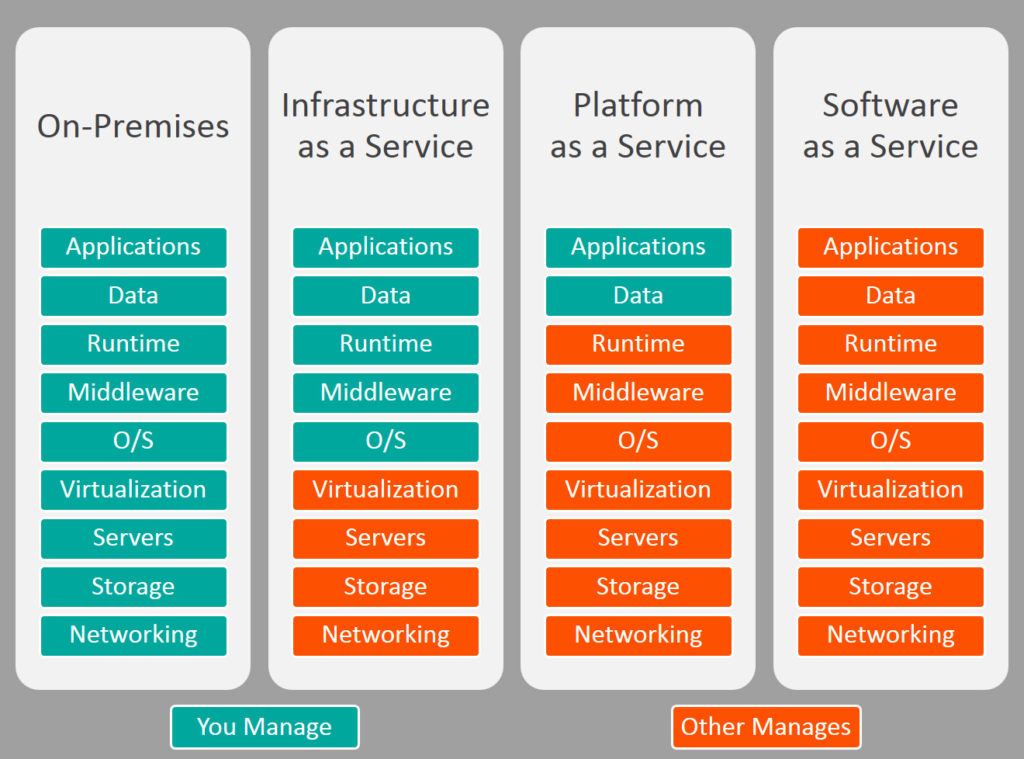
\includegraphics[scale=0.3]{cloud.jpg}
    \caption{I Servizi Cloud}
    \label{fg:cloud.jpg}
  \end{center}
\end{figure}
\subsection{Grid-Computing}
In un'architettura basata sul Grid-Computing, le risorse informatiche(anche qui di qualunque tipo ma sopratutto di calcolo e memorizzazione) possono essere messe a disposizione dell'utente per risolvere determinati problemi (di solito di natura molto complessa dal punto di vista del tempo e dello spazio). La maggiore differenza con il Cloud la si evince su come è costruita l'infrastruttura dei nodi. I nodi come dice stesso la parola formano una specie di "griglia" ma in quest'ultima la rete che collega i vari nodi è formata da una rete locale e questo comporta un migliore aumento delle prestazioni a causa del basso consumo a livello comunicativo che i nodi devono effettuare per spedire i dati attraverso la rete. Questa infrastruttura è quella che viene comunemente chiamata \textbf{data center} e vari sono stati negli anni le possibili soluzioni architetturali che potessero permettere di aggiungere nuovo hardware con facilità (quindi facilitare la scalabilità delle risorse), facili da gestire in fase di manutenzione e installazione del sistema operativo il tutto senza compromettere le prestazioni. 
\section{Modello Distribuito e Modello Shared Memory}
La domanda che ci si pone immediatamente è la seguente: Perché eseguire calcoli in ambiente distribuito piuttosto che in shared memory? La risposta la si ottiene se si guarda indietro alla storia dell'informatica e del calcolo parallelo. I primi modelli di macchine parallele sono state ideate tra gli anni cinquanta e sessanta per poi raggiungere il loro periodo d'oro tra gli anni settanta e ottanta con l'avvento di macchine come Cry-1, Cry-2, Encore che avevano un'enorme potenza oltre all'enorme quantità di denaro necessario per comprarle e manutenerle. Queste macchine ormai sono un ricordo lontano e la causa del loro fallimento è riconducibile a vari fattori:
\begin{description}
    \item [Fisico:] Come ci dice la "Legge" di Moore il numero di transistor all'interno di un processore raddoppia all'incirca ogni 18 mesi. Sappiamo però che questo incremento non sarà, se non è già, più possibile perché non si può ridurre la grandezza dei transistor oltre una certa soglia ($14nm$ anche se sappiamo che Intel è riuscita ad arrivare fino ad $11nm$) per non provocare problemi legati al \textbf{\textit{thermal noise}}\footnote{Detto anche Rumore Termico è la forma più comune di degradazione di un segnale che coinvolge tutte forme di dissipazione del calore con una temperatura diversa dallo zero assoluto}. 
    \item [Sviluppo:] Aumentare il grado di multiprogrammazione tramite l'ausilio di thread ha sicuramente arginato in parte il problema ma non è sicuramente una soluzione in quanto i limiti imposti dalle architetture shared memory rappresentano comunque un collo di bottiglia che inficia sulle prestazioni. Per tentare di risolvere questo problema allora si è cercato di sfruttare modelli di calcolo parallelo tramite l'ausilio di standard di comunicazione (come ad esempio MPI) che sono una possibile soluzione ma rappresentano uno sforzo non da poco da parte del programmatore che deve esplicitamente decidere quali parti del proprio programma parallelizzare o meno.
    \item[Portabilità:] Macchine del genere avevano sistemi operativi dedicati ed era difficile adattare programmi paralleli su altri architetture dovuto anche alla grande quantità di famiglie di processori che, prima che Intel ed AMD conquistassero il mercato, esistevano e il passaggio ad architetture multi core peggiorò la situazione portando all'estinzione non soltanto queste macchine ma anche un intera famiglia di sistemi operativi Unix-like
\end{description}